    % specifies the documnt class. We usually use article but there are others. 
\documentclass[a4paper,12pt,oneside]{book}              

% these are standard packages used for the math symbols
\usepackage{amsmath,amssymb,amsthm, enumitem, hyperref, tabto} 
\usepackage[T1]{fontenc}
\usepackage[utf8]{inputenc}
\usepackage[english]{babel}
\usepackage{fancyhdr}
\usepackage{wrapfig}
\usepackage{lastpage}
\usepackage[pdftex]{graphicx}
\usepackage[utf8]{inputenc}
\usepackage{graphicx}
\usepackage{float}
\usepackage[absolute,overlay]{textpos}
\graphicspath{ {./Photos/} }
\usepackage{fancyhdr}
\usepackage[top=1in,bottom=1in,right=1in,left=1in]{geometry}
\usepackage{circuitikz}
\usepackage{tikz}
\usepackage{pgfplots}
\usetikzlibrary{decorations.markings,arrows}
\usetikzlibrary{datavisualization}
\usetikzlibrary{datavisualization.formats.functions}
\pgfplotsset{compat=newest}
\usepackage{amsmath}

% These commands below is to make sure the numbering of these are consistent with theorem
% If you are not sure what something means, delete them, build a new file and see the
% difference between the files. You can ignore this part for now.
\newtheorem{theorem}{Theorem}[section]
\newtheorem{conjecture}[theorem]{Conjecture}
\newtheorem{observation}[theorem]{Observation}
\newtheorem{definition}[theorem]{Definition}
\newtheorem{corollary}[theorem]{Corollary}
\newtheorem{lemma}[theorem]{Lemma}
\newtheorem{example}[theorem]{Example}
\newtheorem{remark}[theorem]{Remark}
\newtheorem{notation}[theorem]{Notation}


% Title of your project
\title{%
  \Huge Euler's Formula \\
  \LARGE  The Truth Behind Complex Numbers
  \Large Supplementary Material
  }

% The author command places text right after title
\author{by \\
\Large The NUS High Math Interest Group (MIG) \\
}

\date{\Large April - May 2021}

\begin{document}
\maketitle

\tableofcontents

\part{Amazing Applications of Euler's Formula}
\chapter{The Physics Behind it All}
\section{Introduction}
If you look at it, Physics uses Euler's Formula more so that even Mathematics itself. From something as fundamentally basic as Simple Harmonic Motion to expansive topics like Quantum Mechanics' "Particle in a box" set-up, complex numbers are used most fundamental physical concepts by which we operate.

\section{The Complexity of the Simplest Harmonic Motion}
Simple Harmonic Motion, as a concept, can be very simply explained off-hand by a few equations, as shown:

\[a = -\omega^2 x = \frac{dv}{dt} = \frac{d^2x}{dt^2} \] \\

Effectively, Simple Harmonic Motion operates on a sinusoidal basis, or rather, operates as a product of a $\sin$ or $\cos$ function, as can be mathematically shown by solving the differential equation as follows:

\[\frac{d^2x}{dt^2} = -\omega^2 x \] \\

However, besides this solution of course, you can simply solve this using Exponential Expression. But there is one problem. Normal Exponential Expressions don't work well.

Let's say the solution is given by
\[x = e^{bt} \]
We can now differentiate this to get the velocity:
\[v = b e^{bt} \]
Now, deriving the acceleration, we get:
\[a = b^2 e^{bt} \]
However, we then get that
\begin{align*}
    b^2 &= - \omega^2 \\ \implies \left (\frac{b}{\omega} \right )^2 &= -1
\end{align*} \\
If b is a real number, $b^2 \geq 0$
However, the only way this solution would work is to bring in our favourite imaginary but not imaginary number:
\[\frac{b}{\omega} = i \]
Hence, we have that
\begin{align*}
    \frac{b}{\omega} &= i \\
    b &= i \omega \\
    x &= e ^ { i \omega t } \\
    &= \cos \left ( \omega t \right ) + i \sin \left ( \omega t \right ) \\
    v &= i \omega e ^ { i \omega t } \\
    &= i \omega \cos \left ( \omega t \right ) - \omega \sin \left ( \omega t \right ) \\
    a &= - \omega^2 e ^ { i \omega t } \\
    &= - \omega^2 \cos \left ( \omega t \right ) - i \omega^2 \sin \left ( \omega t \right ) \\
\end{align*}

Let's now try drawing out the argand diagram as shown below:

\begin{center}
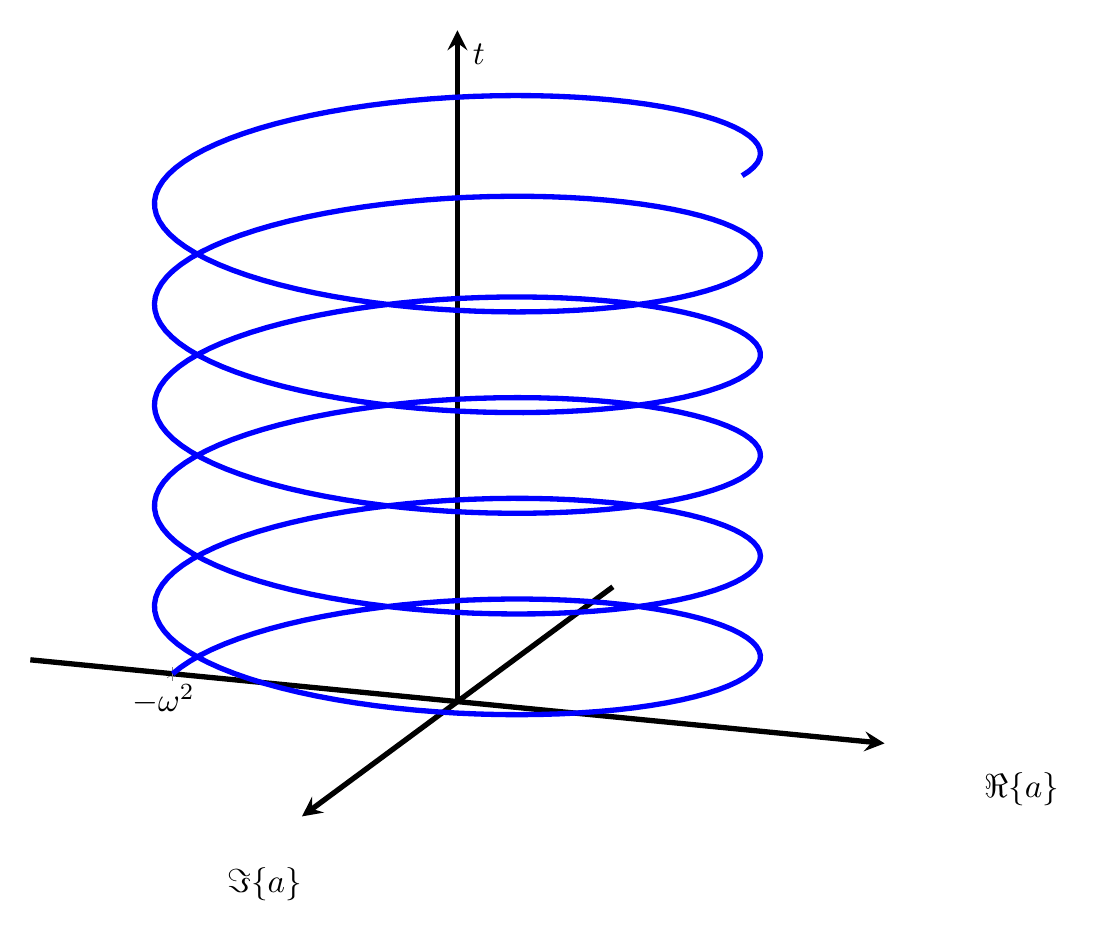
\begin{tikzpicture}[scale=1.2]
\begin{axis}[
 view={-20}{-20},
 axis line style = ultra thick,
 axis lines=middle,
 zmax=80,
  ymax=1.5,
  xmax=1.5,
   xmin=-1.5,
   ymin=-1.5,
 height=12cm,
        xtick = {-1},
        xticklabels = {$-\omega^2$},
 ytick=\empty,
 ztick=\empty,
 clip=false,
 x label style={at={(axis cs:2,0.051)},anchor=north},
   xlabel={$\Re\{a\}$},
 y label style={at={(axis cs:0.05,2)},anchor=north},
   ylabel={$\Im\{a\}$},
 z label style={at={(axis cs:0.075,0,80)},anchor=north},
   zlabel={$t$},
]
\addplot3+[domain=0:11*pi,samples=500,samples y=0,no marks,ultra thick] 
({-cos(deg(x))}, 
{-sin(deg(x))}, 
{6*x/(pi)});
\end{axis}

\end{tikzpicture}
\end{center}

As is noticeable from the above plot, if we were to simply map this plot on the $\Re{a}$ and $t$, we notice a sinusoidal wave formation as shown below:

\begin{center}
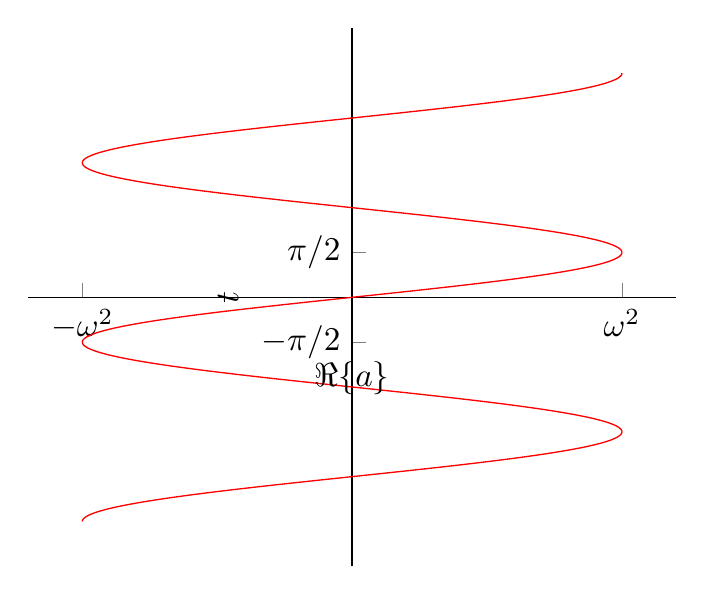
\begin{tikzpicture}[scale=1.2]
  \begin{axis}[domain=-1:1, samples=4000, axis lines*=middle, xtick={-1,1}, ytick={-90,90}, xticklabels={$-\omega^2$,$\omega^2$}, yticklabels={$-\pi$/2,$\pi$/2},
  xlabel={$\Re\{a\}$},
  ylabel={$t$}
  ]
    \addplot[color = red]  {asin(x)-360};
    \addplot[color = red]  {asin(-x)-180};
    \addplot[color = red]  {asin(x)};
    \addplot[color = red]  {asin(-x)+180};
    \addplot[color = red]  {asin(x)+360};
      \end{axis}
\end{tikzpicture}
\end{center}

This is the exact motion in which a wave moves, i.e. a circle is simply dissipating a harmonic wave. Since a Simple Harmonic Motion Oscillator is known to do this too, we realise that Simple Harmonic Motion is analogous to a rotation on the Argand Diagram. In fact, we denote this motion as a \textbf{phasor}.


\section{Phase Through Something: What is a Phasor}

A Phasor is a mathematical concept often used in Physics and Engineering that is often used to represent a sinusoidal wave function with the help of a circle on the Argand Diagram. Surprisingly, the entire concept of a phasor is based on Euler's Formula, hence it allows us to use the Euler Notation to represent a legitimate wave. \\

\subsection{The Wave Function: Escape from Schrödinger}

As we know, the \textbf{Wave Function} is defined as follows.

\[ \psi(x, t) = A \cos(kx - \omega t + \phi) \]

This is a generic equation used for the propagation of waves, where we state the following mathematical definitions:

\begin{align*}
    k &= \frac{2\pi}{\lambda} \\
    \omega &= \frac{2\pi}{T}
\end{align*}

This is an incredibly important formula, since it is able to explain not only the apparent movement in simple harmonic motion at it's finest but it is also able to extend the concept of really any sinusoidal pattern, whether it be transverse waves like electromagnetic waves or longitude waves like sound waves, or even the harmonic motion often found in systems like that of Alternating Current. \\

 \newpage
In fact, we can plot this wave against both distance and time, as shown below:

\begin{center}
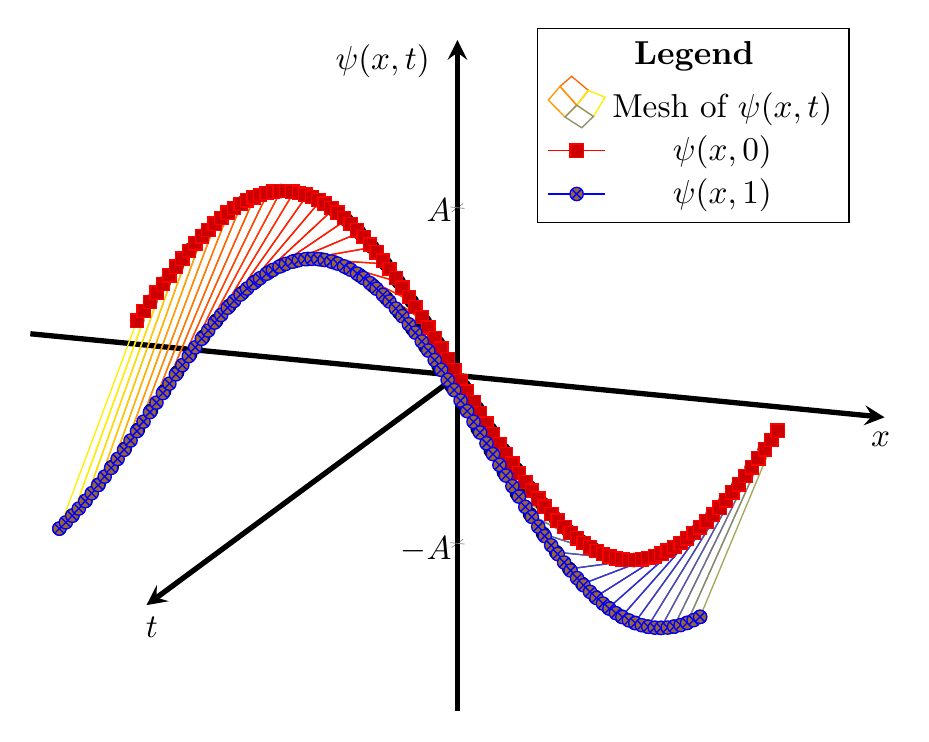
\begin{tikzpicture}[scale=1.2]
   \begin{axis}[
    view={-20}{-20},
   axis line style = ultra thick,
   axis lines = middle,
   height=12cm,
     clip=false,
 x label style={at={(axis cs:4,0.051,0)},anchor=north},
  xlabel={$x$},
 y label style={at={(axis cs:0.05,4,0)},anchor=north},
  ylabel={$t$},
 z label style={at={(axis cs:-0.7,0,2)},anchor=north},
  zlabel={$\psi(x, t)$},
  xtick=\empty,
  ytick=\empty,
  ztick={-1,1},
  zticklabels={$-A$,$A$},
   samples=8,zmin=-2,zmax=2,xmin=-4,xmax=4,ymin=0,ymax=4,
   legend pos = north east
   ]
   \addlegendimage{empty legend}
    %\addplot3[domain=-300:300] {cos(x-y)};
    \addplot3+ [
    domain=-3:3,
    domain y = 0:1,
    samples = 50,
    samples y = 2, mesh] {-sin(deg(x-y))};
    \addplot3+ [domain=-3:3, samples = 100, samples y = 0] {-sin(deg(x))};
    \addplot3+[samples y=0, domain=-3:3, samples=100, variable=\x, blue] ( {x}, {1}, {-sin(deg(x-1))} );
    
    \addlegendentry{\hspace{-.6cm}\textbf{Legend}}
   \addlegendentry{Mesh of $\psi(x, t)$}
   \addlegendentry{$\psi(x, 0)$}
   \addlegendentry{$\psi(x, 1)$}
   \end{axis}
\end{tikzpicture}
\end{center}

However, considering waves as simply a harmonic oscillator operating in 3D space, as we have somewhat previously established, we note that introducing an Argand representation is very much a possible interpretation of a wave. While it is pretty much impossible to really plot the Argand intepretation of the wave against both distance and time, since this would entail an idealistic 4-vector, it is still reasonable to interpret it as an Electromagnetic wave. \\

In an electromagnetic wave, the photon particle flows through a strange sinusoidal formation, since the residual effects of the electric and magnetic fields lead to a rather confusing albeit interesting wave formation. The following shows an example of this graph:

% Electromagnetic wave - colored
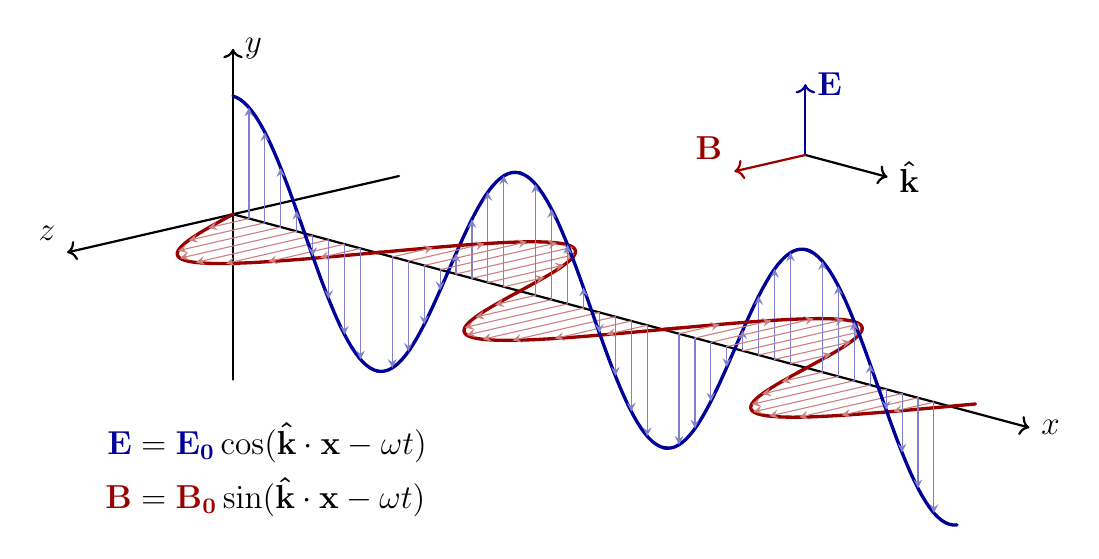
\begin{tikzpicture}[x=(-15:1.2), y=(90:1.0), z=(-150:1.0),
                    line cap=round, line join=round,
                    axis/.style={black, thick,->},
                    vector/.style={>=stealth,->}]
  \large
  \def\A{1.5}
  \def\nNodes{5} % use even number
  \def\nVectorsPerNode{8}
  \def\N{\nNodes*40}
  \def\xmax{\nNodes*pi/2*1.01}
  \pgfmathsetmacro\nVectors{(\nVectorsPerNode+1)*\nNodes}
 
  \def\vE{{\color{black!40!blue}\mathbf{E}}}
  \def\vB{{\color{black!40!red}\mathbf{B}}}
  \def\vk{\mathbf{\hat{k}}}
 
  \def\drawENode{ % draw E node and vectors with some offset
    \draw[black!40!blue,very thick,variable=\t,domain=\iOffset*pi/2:(\iOffset+1)*pi/2*1.01,samples=40]
      plot (\t,{\A*cos(\t*360/pi)},0);
    \foreach \k [evaluate={\t=\k*pi/2/(\nVectorsPerNode+1);
                           \angle=\k*90/(\nVectorsPerNode+1);}]
                in {1,...,\nVectorsPerNode}{
      \draw[vector,black!40!blue!50]  (\iOffset*pi/2+\t,0,0) -- ++(0,{\A*cos(2*\angle+\iOffset*180)},0);
    }
  }
  \def\drawBNode{ % draw B node and vectors with some offset
    \draw[black!40!red,very thick,variable=\t,domain=\iOffset*pi/2:(\iOffset+1)*pi/2*1.01,samples=40]
      plot (\t,0,{\A*sin(\t*360/pi)});
    \foreach \k [evaluate={\t=\k*pi/2/(\nVectorsPerNode+1);
                           \angle=\k*90/(\nVectorsPerNode+1);}]
                in {1,...,\nVectorsPerNode}{
      \draw[vector,black!40!red!50]  (\iOffset*pi/2+\t,0,0) -- ++(0,0,{\A*sin(2*\angle+\iOffset*180)});
    }
  }
 
  % main axes
  \draw[axis] (0,0,0) -- ++(\xmax*1.1,0,0) node[right] {$x$};
  \draw[axis] (0,-\A*1.4,0) -- (0,\A*1.4,0) node[right] {$y$};
  \draw[axis] (0,0,-\A*1.4) -- (0,0,\A*1.4) node[above left] {$z$};
 
  % small axes
  \def\xOffset{{(\nNodes-2)*pi/2}}
  \def\yOffset{\A*1.2}
  \def\zOffset{\A*1.2}
  \draw[axis,black] (\xOffset,\yOffset,-\zOffset) -- ++(\A*0.6,0,0) node[right,align=center] {$\mathbf{\hat{k}}$}; %\\propagation
  \draw[axis,black!40!blue]  (\xOffset,\yOffset,-\zOffset) -- ++(0,\A*0.6,0) node[right] {$\mathbf{E}$};
  \draw[axis,black!40!red]   (\xOffset,\yOffset,-\zOffset) -- ++(0,0,\A*0.6) node[above left] {$\mathbf{B}$};
 
  % equation
  \node[above right] at (\xOffset,-0.5*\yOffset,4*\zOffset)
    {$\begin{aligned}
      \vE &= {\color{black!40!blue}\mathbf{E_0}}\cos(\vk\cdot\mathbf{x}-\omega t)\\
      \vB &= {\color{black!40!red} \mathbf{B_0}}\sin(\vk\cdot\mathbf{x}-\omega t)\\
      \end{aligned}$};
 
  % draw (anti-)nodes
  \foreach \iNode [evaluate={\iOffset=\iNode-1;}] in {1,...,\nNodes}{
    \ifodd\iNode \drawBNode \drawENode % E overlaps B
    \else        \drawENode \drawBNode % B overlaps E
    \fi
  }
 
\end{tikzpicture}

\newpage

When you superpose these two waves, we get the following vector formation, which is a helix.
 
% Electromagnetic wave - circular polarization
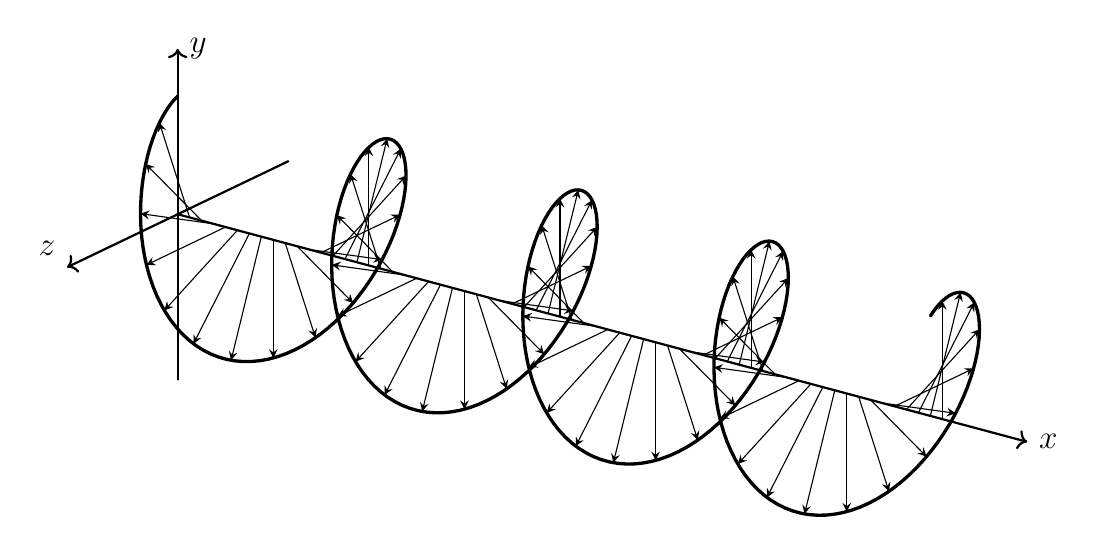
\begin{tikzpicture}[x=(-15:0.8), y=(90:1.0), z=(-150:1.0),
                    line cap=round, line join=round,
                    axis/.style={black, thick,->},
                    vector/.style={>=stealth,->}]
  \large
  \def\A{1.5}
  \def\nNodes{8} % use even number
  \def\nVectorsPerNode{8}
  \def\N{\nNodes*40}
  \def\xmax{\nNodes*pi/2*1.01}
  \pgfmathsetmacro\nVectors{\nVectorsPerNode*\nNodes}
 
  \def\vE{\mathbf{E}}
  \def\vB{\mathbf{B}}
  \def\vk{\mathbf{\hat{k}}}
 
  % main axes
  \draw[axis] (0,0,0) -- ++(\xmax*1.1,0,0) node[right] {$x$};
  \draw[axis] (0,-\A*1.4,0) -- (0,\A*1.4,0) node[right] {$y$};
  \draw[axis] (0,0,-\A*1.4) -- (0,0,\A*1.4) node[above left] {$z$};
 
  % waves
  \draw[very thick,variable=\t,domain=0:\nNodes*pi/2*1.01,samples=\N]
    plot (\t,{\A*cos(\t*360/pi)},{\A*sin(\t*360/pi)});
 
  % draw vectors
  \foreach \k [evaluate={\t=\k*pi/2/\nVectorsPerNode;
                         \angle=\k*90/\nVectorsPerNode;}]
              in {1,...,\nVectors}{
    \draw[vector] (\t,0,0) -- ++(0,{\A*cos(2*\angle)},{\A*sin(2*\angle)});
  }
 
\end{tikzpicture}
 
This is another way of depicting a wave, with $y$ representing $\Re(\Psi) = \psi$ and $z$ representing $\Im(\Psi)$. This, of course, is a snapshot wave, since time is not a factor, but notably, we can now represent $\Psi(x, t)$ as follows:

\[ \Psi(x, t) = A \left( \cos(kx - \omega t + \phi) + i \sin(kx - \omega t + \phi) \right) = A e^{i \left(kx - \omega t + \phi \right)} \]

Here, we of course assume that $B_0 = E_0$. This is an interesting way of depicting waves using a phasor of sorts. Notably, if we consider an alternative wave that starts at 0, as shown below:

\[ \delta(x, t) = A \sin(kx - \omega t + \phi) \]

From here, we try to derive a function $\Delta(x, t)$ as follows:
\[ \Re{\left(\Delta(x, t)\right)} = A \sin(kx - \omega t + \phi) \]

We can note the following:
\begin{align*}
    \Psi(x, t) &= A e^{i \left(kx - \omega t + \phi \right)} \\
    &= A \cos(kx - \omega t + \phi) + iA \sin(kx - \omega t + \phi) \\
    \frac{\Psi(x, t)}{i} &= \frac{A}{i} \cos(kx - \omega t + \phi) + A \sin(kx - \omega t + \phi) \\
    &= A \sin(kx - \omega t + \phi) - iA \cos(kx - \omega t + \phi) \\
    \Re{\left(\frac{\Psi(x, t)}{i}\right)} &= A \sin(kx - \omega t + \phi) \\
    \Delta(x, t) &= \frac{\Psi(x, t)}{i} \\
    &= A \frac{e^{i \left(kx - \omega t + \phi \right)}}{e^{i\frac{\pi}{2}}} \\
    &= A e^{i \left(kx - \omega t + \phi - \frac{\pi}{2} \right)}
\end{align*}

Basically, a sinusoidal function operating on a $\sin$ function is out of phase by $\frac{\pi}{2}$ from a $\cos$ function. As we know,

\begin{center}
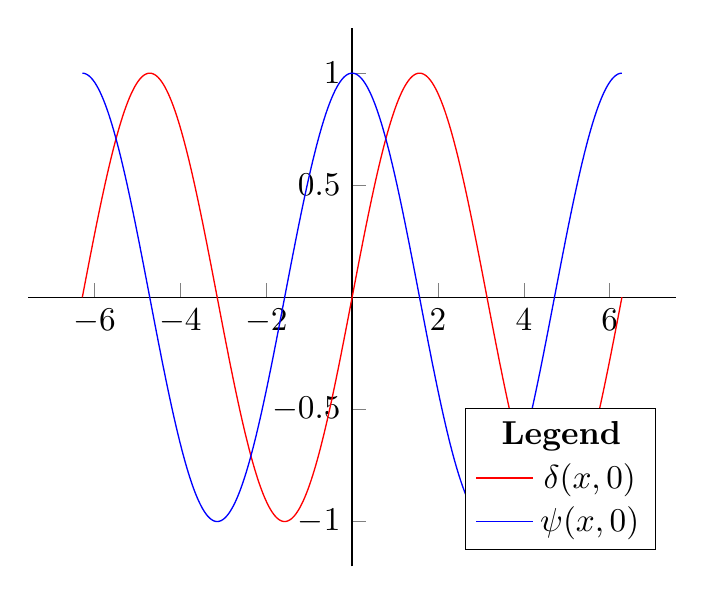
\begin{tikzpicture}[scale=1.2]
  \begin{axis}[domain=-2*pi:2*pi, samples=4000, axis lines*=middle, legend pos=south east]
  \addlegendimage{empty legend}
    \addplot[color = red]  {sin(deg(x))};
    \addplot[color = blue]  {cos(deg(x))};
    \addlegendentry{\hspace{-.6cm}\textbf{Legend}}
   \addlegendentry{$\delta(x, 0)$}
   \addlegendentry{$\psi(x, 0)$}
  \end{axis}
\end{tikzpicture}
\end{center}

In this case, we note that by extension,

\[ \Re{\left(\Delta(x, t)\right)} = \cos \left(kx - \omega t + \phi - \frac{\pi}{2} \right) = A \sin(kx - \omega t + \phi) \]

From here, we get that:

\[ \sin\theta = \cos \left(\theta - \frac{\pi}{2} \right) \]

This is an actual concept of leading and lagging, which is very much synonymous with phasors (which this materials seems to have lost sight of).

\subsection{The Confusion behind Leading and Lagging}

As we must recall from the transformation of graphs, the $\sin$ function is simply a translation parallel to the x=axis by $\frac{\pi}{2}$ units in the positive direction applied on the $\cos$ function, based on the above function. \\

However, in phasors, this is instead said as the $\sin$ function \textbf{lags} the $\cos$ function by $\frac{\pi}{2}$, or alternatively, the $\cos$ function \textbf{leads} the $\sin$ function by $\frac{\pi}{2}$. \\

In phasor terminology, $v_1$ lagging $v_2$ is defined as, in a way, "pushing the other function backward", or rather making the latter function be termed as lagging behind the former. Idealistically, we consider $v_1$ to be the base, and consider $v_2$ relative to $v_1$. As per the graph above, $\cos$ experiences the same signal as $\sin$ beforehand, hence $\cos$ is stuck behind. \\

On the other hand, $v_2$ leading $v_1$, which is basically identical to the above statement, is defined in a similar way, by "pushing the other function forward", or rather making the latter function be termed as being ahead of the former. It's a similar relative motion comparison. \\

While this terminology may seem rather unintuitive, all you really need to know is that this works similar to the translation transformation in the transformation of graphs. Since $v_2$ is leading $v_1$,  $v_2$ is simply $v_1$ transformed by a translation parallel to the x-axis by some $\phi$ units in the negative direction.

\subsection{Superposition in Waves}

Waves perform very specific tests, but in fact superposition is one of the many important ones. For instance, let's say you have a transverse wave of a Wave Function as follows:
\[ \psi_1(x, t) = A \cos(kx - \omega t) \]
And another moving similarly but out of phase as follows:
\[ \psi_2(x, t) = A \sin(kx - \omega t) \]

When these two wave merge, superposition of waves takes place, wherein at any point, the wave function now becomes:
\[ \psi_T(x, t) = A \left(\cos(kx - \omega t) + \sin(kx - \omega t) \right) \]

If you think about this using the general definition of the R formula, we can solve for the function 

\[R \cos(\theta - \alpha) = \cos\theta + \sin\theta \]

As follows (in a very rigorously explicit piece of working the math department would be proud of):

\begin{align*}
    \cos\theta + \sin\theta &= R \cos(\theta - \alpha)  \\
    %&= R \left(\cos\theta\cos\alpha + \sin\theta \sin\alpha \right) \\
    &= R \cos\theta\cos\alpha + R \sin\theta \sin\alpha \\
    R \sin\theta = R \cos\theta &= 1 \implies \tan\theta = 1 \implies \theta = \frac{\pi}{4} \\
    R^2\cos^2\theta = \left(R\cos\theta)\right)^2 &= 1 = R^2\sin^2\theta = \left(R\sin\theta)\right)^2 \\
    %R^2\sin^2\theta = \left(R\sin\theta)\right)^2 &= 1 \\
    R^2\sin^2\theta + R^2\cos^2\theta  &= 2 \implies R^2 = 2 \implies R = \sqrt{2} \\
    \therefore \cos\theta + \sin\theta &= \sqrt{2} \cos \left(\theta - \frac{\pi}{4} \right) 
\end{align*}

From here, we get that:

\[ \psi_T(x, t) = \sqrt{2} A \cos \left(kx - \omega t - \frac{\pi}{4} \right) \]

This would be the generic solution to solve for superposition, but we can also do this same thing in the Euler form. Firstly, we redefine the functions as follows:
\begin{align*}
    \Psi_1(x, t) &= A e^{i \left(kx - \omega t \right)} \\
    \Psi_2(x, t) &= A e^{i \left(kx - \omega t - \frac{\pi}{2} \right)} = A e^{i \left(kx - \omega t \right)} e^{-\frac{\pi}{2}}  \\
    \Psi_T(x, t) &= A e^{i \left(kx - \omega t \right)} + A e^{i \left(kx - \omega t \right)} e^{-\frac{\pi}{2}}  \\
    &= A e^{i \left(kx - \omega t \right)} \left( 1 - i \right) \\
    &= \sqrt{2} A e^{i \left(kx - \omega t \right)} \left(\frac{1}{\sqrt{2}} - i \frac{1}{\sqrt{2}} \right) \\
    &= \sqrt{2} A e^{i \left(kx - \omega t \right)} \left(\cos\left(-\frac{\pi}{4}\right) + i\sin\left(-\frac{\pi}{4}\right) \right) \\
    &= \sqrt{2} A e^{i \left(kx - \omega t \right)} e^{-i\frac{\pi}{4}} \\
    &= \sqrt{2} A e^{i\left(kx - \omega t - \frac{\pi}{4} \right)} \\
    &= \sqrt{2} A \cos\left(kx - \omega t - \frac{\pi}{4} \right) + i\sqrt{2} A \sin\left(kx - \omega t - \frac{\pi}{4} \right)
\end{align*}

This method also allows you to solve simple trigonometric operations and formulae like the R-Formula and the Factor Formulae, which are of course tedious to memorise. Hence, mathematically speaking, this is a much simpler way of doing this. Superposition also involves subtraction waves 


However, the best real definition of a phasor is in \textbf{Alternating Current}, which also operates in a wave-like formation. \\

\newpage
\subsection{Alternating Current: Live Complexity}

In this material, we focus especially on the applications of Euler's Formula in advanced circuitry, where complexity appears to be a major focus. \\

Ever since George Westinghouse and Nikola Tesla's historic revolt against the Edison Electric Light Company's (now General Electric) tyrannical usage of Direct Current (DC) and its adoption of Alternating Current (AC) and transformers as a general part of society's usage of electricity, our usage of electricity has always been sinusoidal in nature. \\

In fact, the electrical socket which you use to charge virtually every electronic device you may have transmits electricity by Alternating Current through the infamous "live wire". In Singapore, the electrical socket is rated to 230V, which means that in the standard AC Circuit, with the live socket as the AC source, the "wave equation", so to speak, is as follows:

\[ V(t) = V_{max} \cos(\omega t + \phi) \]


% \begin{center}
% \begin{tikzpicture}[samples=100, >=latex]
%     \def\Alpha{60}
%     \def\AlphaRad{3.141592654/3}
%     \def\VoltageMax{2.7}
%     \def\CurrentMax{1.8}
%     \def\Voltage{{\VoltageMax*sin(\Alpha)}}
%     \def\Current{{\CurrentMax*sin(\Alpha)}}
%     %%%%%%%%%%%%%%%%%%%%%%%%%%%%%%%%%%%%%%%%%%%%%%%%%%%%%%%%%%
%     \draw[very thin,color=gray] (-.1,-3.1) grid (7.1,3.1);
%     \draw[->, >=latex, color=green!50!black] (-.2,0) -- (7.3,0) node[right] {$\omega t$};
%     \draw[->, >=latex, color=green!50!black] (0,-3.2) -- (0,3.3) node[left] {};
%     \draw (1.570795,0) node[below]{$\frac{\pi}{2}$};
%     \draw (3.14159,0) node[below]{${\pi}$};
%     \draw (4.71238898,0) node[below]{$\frac{3\pi}{2}$};
%     \draw (6.283185307,0) node[below]{${2\pi}$};
%     \draw (-4,0) circle (3cm);
%     \draw[-] (-7.2,0) -- (-.8,0);
%     \draw[-] (-4,-3.6) -- (-4,3.6);
%     %%%%%%%%%%%%%%%%%%%%%%%%%%%%%%%%%%%%%%%%%%%%%%%%%%%%%%%%%%

%     % voltage
%     \draw[color=blue!90!white, very thick] plot[id=voltage, domain=0:7] function{\VoltageMax*sin(x)} node[right] {$V(t)$};
%     % voltage circle
%     \draw[color=blue!90!white, loosely dashed] (-4,0) circle (\VoltageMax cm);
%     % angle
%     \draw[color=green!50!black, thick] (\AlphaRad, \Voltage)--(\AlphaRad,\Current) node[below=18pt] {$\alpha$};
%     % angle in the circle
%     \filldraw[fill=green!20,draw=green!50!black] (-4,0) -- (-3,0) arc (0:\Alpha:1) -- cycle node[right] {$\alpha$};
%     % voltage pointer
%     \draw[<-,color=blue!90!white, very thick] (\Alpha:\VoltageMax)++(-4,0) --(-4,0);
%     \draw[color=blue!90!white,  dashed] (\Alpha:\VoltageMax)++(-4,0) -- (\AlphaRad,\Voltage);
%     % current
%     \draw[color=red!90!white, very thick] plot[id=current, domain=0:7] function{\CurrentMax*sin(x)} node[right] {$I(t)$};		
%     % current circle
%     \draw[color=red!90!white, loosely dashed]    (-4,0) circle (\CurrentMax cm);
%     % current pointer
%     \draw[<-,color=red!90!white, very thick] (\Alpha:\CurrentMax)++(-4,0) --(-4,0);
%     \draw[color=red!90!white,  dashed](\Alpha:\CurrentMax)++(-4,0) -- (\AlphaRad,\Current);
%     % phase difference
%     % angular velocity \omega
%     \draw[->, xshift=-4cm]  (120:2.4cm) arc (120:170:2) node[below] {$\omega$};
% \end{tikzpicture}
% \end{center}

% \bibliographystyle{acm}
% \bibliography{MainBib.bib}

\end{document}
